\documentclass{elsarticle}
\usepackage{graphicx}
%\usepackage{multicol}
%\usepackage{footmisc}
\usepackage{amstext}
\usepackage{amsmath}
\usepackage{amssymb}
\usepackage{amsthm}
\usepackage[english]{babel}
%\usepackage[official,right]{eurosym}
\selectlanguage{english}
\hyphenation{ExecEngine}
\newtheorem{lemma}{Lemma}
\def\Events{{\mathit E}}
\begin{document}
% Ampersand -----------------------------------------------------------

%\def\id#1{\text{\it #1\/}}
\newcommand{\id}[1]{\text{\it #1\/}}
\newcommand{\code}[1]{\text{\tt\small #1}}
\newcommand{\stmtText}[1]{``{\small\tt #1}''}
\newcommand{\dom}[1]{\id{dom}(#1)}
\newcommand{\cod}[1]{\id{cod}(#1)}
\renewcommand{\int}[2]{\id{inter}(#1,#2)}
\newcommand{\relsIn}[1]{\id{relsIn}(#1)}    % maps a Term to a set of Relations
\newcommand{\maintain}{\id{maint}}
\newcommand{\pop}[2]{\id{pop}_{#1}(#2)}
\newcommand{\inst}{\id{inst}}
\newcommand{\relname}[1]{\id{relname}(#1)}
\newcommand{\src}[1]{\id{src}(#1)}
\newcommand{\tgt}[1]{\id{tgt}(#1)}
\newcommand{\sat}[2]{\id{sat}_{#1}(#2)}
\newcommand{\viol}[2]{\id{viol}_{#1}(#2)}
\newcommand{\sign}[1]{\id{sign}(#1)}
\newcommand{\powerset}[1]{\cal{P}\{#1\}}
\newcommand{\theCode}{\url{http://cs.ru.nl/~B.Joosten/ampTypes/}}
\newcommand{\la}{\langle}
\newcommand{\ra}{\rangle}
\newcommand{\full}{V}
\newcommand{\declare}[3]{\id{#1}_{\pair{#2}{#3}}}
\newcommand{\subst}[3]{#3_{[#1\rightarrow #2]}}
\newcommand{\fullt}[2]{V_{\pair{#1}{#2}}}
\newcommand{\iden}{I}
\newcommand{\ident}[1]{I_{\id{#1}}}
\newcommand{\expr}[3]{(#1)_{#2\times #3}}
\newcommand{\pair}[2]{\la{#1},{#2}\ra}
\newcommand{\Pair}[2]{#1\times#2}
\newcommand{\pairs}[1]{\id{pairs}(#1)}
\newcommand{\triple}[3]{\la{#1},{#2},{#3}\ra}
\newcommand{\quadruple}[4]{\la{#1},{#2},{#3},{#4}\ra}
\newcommand{\atom}[1]{{\tt\small #1}}
\newcommand{\atoms}{\mathcal{A}}
\newcommand{\Atoms}{\mathbb{A}}
\newcommand{\concept}[1]{{\tt\small #1}}
\newcommand{\concepts}{\mathcal{C}}
\newcommand{\Concepts}{\mathbb{C}}
\newcommand{\decls}{\mathcal{D}}  %% names of relations
\newcommand{\rels}{\mathcal{R}}   %% all relations
\newcommand{\Rels}{\mathbb{R}}   %% all relations
\newcommand{\relations}{\mathcal{M}} % representing terms. M is a subset of R.
\newcommand{\triples}{\mathcal{T}}
\newcommand{\Triples}{\mathbb{T}}
\newcommand{\Triple}[3]{#1\times#2\times#3}
\newcommand{\vertices}{N}
\newcommand{\rules}{\mathcal{U}}
\newcommand{\Rules}{\mathbb{U}}
\newcommand{\specrules}{\mathcal{S}}
\newcommand{\roles}{\mathcal{O}}
\newcommand{\Events}{{\mathit E}}
\newcommand{\dataset}{\mathscr{D}}
\newcommand{\Dataset}{\mathbb{D}}
\newcommand{\schema}{\mathscr{Z}}
\newcommand{\functionality}{\mathscr{F}}
\newcommand{\select}[2]{\id{select}_{#1}\{{#2}\}}
\newcommand{\migrsys}{\mathscr{M}}
\newcommand{\infsys}{\mathscr{S}}
\newcommand{\tf}[1]{\mathscr{T}(#1)}
\newcommand{\ptf}[1]{\mathscr{T}'(#1)}
\newcommand{\ti}[1]{\mathscr{I}(#1)}
\newcommand{\tic}[1]{I_{\cal C}(#1)}
\newcommand{\relAdd}{\dagger}
\newcommand{\flip}[1]{{#1}^\smallsmile} %formerly:  {#1}^\backsim
\newcommand{\kleeneplus}[1]{{#1}^+}
\newcommand{\kleenestar}[1]{{#1}^*}
\newcommand{\cmpl}[1]{\overline{#1}}
\newcommand{\rel}{\times}
\newcommand{\compose}{;}
\newcommand{\subs}{\subseteq}%{\models}
\newcommand{\fun}{\rightarrow}
\newcommand{\isa}{\preceq}
%\newcommand{\isaClos}{\sqsubseteq}
\newcommand{\typetest}{?}
\newcommand{\meet}{\sqcap}
\newcommand{\join}{\sqcup}
\newcommand{\Meet}{\bigsqcap}
\newcommand{\Moin}{\bigsqcup} % because LaTeX has already defined command \Join.
\newcommand{\order}{\ominus}
\newcommand{\anything}{\top}
\newcommand{\nothing}{\bot}
\newcommand{\rewriteto}{\rightarrow}
\newcommand{\calc}{\implies}
\newcommand{\alland}{\bigwedge}
\newcommand{\mph}[3]{#1_{#2\times #3}}
\newcommand{\mphu}[1]{#1_{\univ\times\univ}}

%-----------------------------------------
\newcommand{\kse}{\hspace*{1.7em}}
\newcommand{\ksf}{\hspace*{1em}}
\newcommand{\ksg}{\hspace*{1em}}
\newenvironment{derivation}{\begin{tabbing}\kse \= \ksf \= \ksg \= \kill}{\end{tabbing}}
\newtheorem{definition}{Definition}
\newcommand{\term}[1]{\>\>\(#1\)\\[1ex]}
\newcommand{\rela}[2]{\>\(#1\)\>\>\{ \ #2 \ \}\\[1ex]}
\newcommand{\weg}[1]{}

\def\define#1{\label{dfn:#1}{\em #1}\index{#1}}
\def\definem#1{\label{dfn:#1}{\em #1}\index{#1}\marge{#1}}
\newcommand{\marg}[1]{\index{#1}\marge{#1}}


% TODO Bas:
% - verhaal over incrementeel fouten oplossen (fouten staan al in artikel)

% TODO Algemeen:
% - type van triple-set en atom-set definieren zodat viol_u ?->P(?x?)
%   (Bas: ik heb foute types weggehaald, maar dit nog niet gedefinieerd)
% - nieuwe populatie na de disjoint union zou de populatie met ENFORCE regels toegepast moeten zijn
%  (en in het bijzonder de ISA regels)

% TODO Stef:
% - stukje literatuuronderzoek
% https://ieeexplore.ieee.org/abstract/document/7445334?casa_token=ECzi6XeV2ncAAAAA:KhWzB8XBFOUJ0C6AD-XjX_ryuA9ARvTd3gm6RR-ZNiR8sZ1858FJpQ7zKQhkAZDlv8IjPdgD
% https://ieeexplore.ieee.org/abstract/document/8549944?casa_token=9qiGqNzh2Q0AAAAA:C-cYogExB35nGxQdxLcdBh4JoLNvM0OHedAMhCbB5V4kb4_6nzHUvc23xSJbeoBu67LSiz-Y
% https://citeseerx.ist.psu.edu/viewdoc/download?doi=10.1.1.651.9298&rep=rep1&type=pdf
% https://www.scirp.org/html/4-7800724_106592.htm
% https://www.researchgate.net/profile/Ranjana-Badre/publication/318665687_GUI_for_Data_Migration_and_Query_Conversion/links/5b45bbea0f7e9b1c722386e5/GUI-for-Data-Migration-and-Query-Conversion.pdf
% https://journal3.uin-alauddin.ac.id/index.php/literatify/article/view/12567



\title{A Theory for Data Migration of Information Systems}
\author[ou,ordina]{Stef Joosten\fnref{fn1}}
\ead{stef.joosten@ou.nl}
\author[umn]{Sebastiaan Joosten\fnref{fn2}}
\address[ou]{Open Universiteit Nederland, Heerlen, the Netherlands}
\address[ordina]{Ordina NV, Nieuwegein, the Netherlands}
\address[umn]{University of Minnesota, Minneapolis, USA}
\fntext[fn1]{ORCID 0000-0001-8308-0189}
\fntext[fn2]{ORCID 0000-0002-6590-6220}

\begin{abstract}
   The Ampersand project has provided the theory and tools to generate semantic information systems from an algebraic specification.
   However, information systems in practice may change repeatedly after their maiden deployment.
   Changes that affect the data model typically result in a data migration.
   In such cases, simply regenerating the system is not enough because it would reset the database to its initial state (deleting all data gathered so far).
   Data migration aims at preserving the data as much as possible.
   Typically, migration involves transferring the old data to the new system while preserving the semantics as much as possible.

   In this contribution we develop a theory for reliable data migration that aims at automating it as much as possible,
   to enable more frequent migrations.
   The ultimate target is to generate a migration from two specifications: the as-is specification and the to-be specification.
   A software generator that embodies this theory is subject of future research.
\end{abstract}

\begin{keyword}
relation algebra\sep software development\sep data migration\sep software migration\sep Ampersand
\end{keyword}
\maketitle

\section{Introduction}
\label{sct:Introduction}
   Our research focuses on generating information systems incrementally,
   especially on the data migration aspect of it.
   The reason that we believe in generating information systems is to prevent human errors as early as possible in the build chain:
   A mistake not made cannot propagate into production.
   Incremental generation of information systems poses specific requirements to data migration.
   For instance, if a data migration is not for incremental generation,
   e.g.~\cite{Gholami2016,Bisbal1999},
   preserving the functionality can be useful to avoid introducing new errors in an otherwise error-prone process.
   For incremental generation, however, preserving the functionality is not an option.
   To change the functionality is the very purpose and the data migration must behave accordingly.
   So, we must make sure to use methods for data migration that are specifically meant for incrementally generating information systems.
   
   Data migration occurs when an as-is information system, $\infsys$, is replaced by a to-be information system, $\infsys'$,
   while preserving the meaning of the data from $\infsys$ as much as possible.
   Just copying the set of data from $\infsys$ to $\infsys'$ is obviously wrong if the schemas of both information systems differ.
   Information systems are typically used by distributed actors (both users and computers) who continually work with data.
   Information system $\infsys$ contains a dataset $\dataset_{\infsys}$, which represents the state of the system.
   (In the sequel we may just write $\dataset$ if the corresponding information system is either obvious or irrelevant.)
   Every event that an actor causes in information system $\infsys$ may change its state $\dataset$.

   Much like~\cite{Spivak2012}, our work assumes that the semantics of the as-is dataset is encoded in its schema,
   so we can be explicit about ``preserving the meaning as much as possible''.
   The schema $\schema_{\infsys}$ of an information system $\infsys$ is basically a set of constraints on its dataset $\dataset$.
   (We will denote the schema just as $\schema$ if the information system is obvious or irrelevant to know.)
   In contrast with earlier work, e.g.~\cite{Thalheim2013}, we assume that the dataset satisfies all semantic constraints in the schema.
   This is possible because we use a compiler, Ampersand~\cite{Joosten-JLAMP2018},
   that generates an information system that keeps all semantic constraints satisfied at all times.
   As a consequence, it contains only data pollution that is not already captured by any of the constraints mentioned in the schema.
   Remaining data pollution must therefore be captured in constraints in the schema of the to-be information system $\infsys'$,
   so it can guard those new constraints from the moment $\infsys'$ is in production.
   In the meantime, the migration engineer must ensure that $\infsys'$ can start with data that satisfies all constraints in its schema.

   We believe that information systems should be released into production in small increments,
   to obtain shorter release cycles, more frequent releases, and thus a more agile software development process%
   \footnote{These effects can be measured in terms of DevOps metrics such as
   deployment frequency,
   reliability of deployments, and
   change failure rate~\cite{DevOps2021}.}.
   In practice, more frequent updates require that updates have zero down-time.
   Extra complications arise from accumulated data pollution in the as-is information system.
   So, the theory we develop in this paper must lead to tools that satisfy such practical requirements as
   zero down-time updates and ways to cope with data pollution.
   That will help agile teams today to automate their software processes further.

   Automating data migrations, however, has its limits.
   If the semantics encoded in the to-be schema $\schema'$ differs from the as-is schema $\schema$,
   a migration engineer must make choices on how to interpret existing data in the new schema.
   She may even want to adapt data of which the constraints in the schema have not changed.
   This requires a third schema, $\schema_m$, which specifies the migration itself.
   We generate $\schema_m$ in the form of source code, so the migration engineer can change everything she wants to suit the particulars of the data migration.
   In the sequel, automation of data migration means to generate the schema $\schema_m$.

   The benefits of automating data migrations work in two directions.
   The automation itself saves effort and errors,
   contributing to more frequent and smaller releases.
   Smaller and faster releases also mean smaller migrations
   and therefore a smaller difference between $\infsys$ and $\infsys'$.
   The smaller that difference, the simpler the migration and the more of it can be automated.

   The contribution of this paper is to derive a migration schema $\schema_m$ from an existing information system $\infsys$
   (which has its own $\schema$ and $\dataset$) and a to-be schema $\schema'$.
   A formal understanding of data migration will help to automate data migrations correctly and reliably.
   Our theory is based on the following assumptions:
\begin{itemize}
   \item the as-is data set may be polluted, but it satisfies its schema;
   \item the data migration may require human interaction, which may take time;
   \item the part of the data that does not change in $\schema'$ can be migrated automatically;
   \item the meaning of data must be preserved;
   \item the business must continu during the migration without interruption;
   \item the part of the migration that can be automated is usually not sufficient;
         it takes additional human creativity to complete the migration specification;
   \item there is a compiler to generate an information system from a given schema.
         In this work, we use the Ampersand compiler for that purpose.
\end{itemize}

\section{Migration steps}
   A smooth migration from an old system to a new system would go as follows:
   Launch the new system in parallel to the old, copy data from the old to the new system, and have everyone use the new system.
   However, numerous issues might impede that plan.
   The following examples illustrate the practical issues that may occur:
\begin{enumerate}
\item Data required in the new system is missing in the old system.
   There may be no way in the old system to enter that data.
   An example could be that every reimbursement form needs to have an address associated to it to mail the check to, but address information is not stored in the old system:
   The old system required the reimbursement office to look up employee's addresses from a hand-written list they had on their desk.
\item Data in the old system is wrong but cannot be corrected there due to how the old system was designed.
   An example is if the old system only allows approvals to be entered as the current user, and the CEO insists that her administrative staff enters his approvals into the system for her.
   This may result in approvals being entered as admin staff, where it was really the CEO making the approval.
\item Data in the old system does not satisfy invariants of the new system.
   There may be no way in the old system of making the data satisfy those invariants. We can use the same example as in the previous bullet point, but add the requirement (in the new system) that every purchase above a certain amount needs to be approved by the CEO.
\item A way of entering data into the old system is missing in the new system.
   People or automated processes might rely on these ways of entering data.
   An example could be that when employees turned their computers on or off, an ad-hoc script would automatically clock them in- and out to determine the number of hours they worked.
   A handful of employees still relies on this.
\item Data present in the old system cannot be stored in the new system.
   An example could be that references to physical locations where original receipts are kept are stored in the old system, but the new system relies on scans of receipts and allows the originals to be destroyed or not submitted.
   Until the original receipts are scanned, the old data should be kept.
\end{enumerate}

(@Bas, het volgende zit al in de oplossingen sfeer. Willen we dat hier al doen?)
   To mitigate these issues, we:
   
   \begin{enumerate}
   \item Allow `missing' triples requirements to be ignored during migration.
   \item Allow triples to be migrated while being marked as needing correction.
   \item Allow invariants in the new system to be ignored for certain triples during migration.
   \item Allow continued use of interfaces of the old system, data entered into the old system via those interfaces needs to be continuously copied to the new system.
   \item Retain data in the old system until it can be marked as ready to be phased out.
   \end{enumerate}   

\section{Terminology}
\label{sct:Terminology}
   To migrate data from one information system to another,
   we must define ``information system''.
   In that definition we will single out the dataset as the focal point of a data migration.
   For this reason, we define datasets first.
   We need rules to capture the semantics, so we need to define rules as well.
   After that, we define information systems.

\subsection{Datasets}
\label{sct:Datasets}
   A dataset describes a set of structured data, which is typically stored persistently in a database of some kind.

   Before defining datasets, we must first define the constituent notions of atom, concept, triple, and relation.
   
   Atoms serve as data elements.
   They are values without internal structure of interest, meant to represent data elements in a database.
   From a business perspective, atoms represent concrete items of the world,
   such as \atom{Peter}, \atom{1}, or \atom{the king of France}.
   By convention throughout the remainder of this paper, variables $a$, $b$, and $c$ represent \emph{atoms}.
   The set of atoms is called $\atoms$.
   
   Concepts are names we use during the design of a dataset
   to name a group of atoms of the same type,
   to assign signatures to relations, and thus
   to enable type checking of the dataset.
   For example, you might choose to classify \atom{Peter} as a \concept{Person}, and \atom{074238991} as a \concept{TelephoneNumber}.
   In this example, \concept{Person} and \concept{TelephoneNumber} are concepts.
   We will use variables $A$, $B$, $C$, $D$ to represent concepts.
   The expression $a\ \inst\ A$ means that atom $a$ is an \emph{instance} of concept $A$.
   The set of concepts is called $\concepts$.
   
   We will use triples to represent data.
   This makes our theory valid for any kind of database that triples can represent,
   such as SQL databases, object-oriented databases, graph databases, triple stores, and other no-SQL databases
   Each triple relates two atoms to a relation.
   A triple $\triple{\text{\atom{Peter}}}{\id{phone}}{\text{\atom{074238991}}}$ might mean in practice that
   the ``thing'' that \atom{Peter} refers to has \atom{074238991} as a telephone number.
   This ``meaning from practice'' has no consequences in the formal world.
   We leave it entirely up to a user to attach a practical meaning to a triple.
   In this paper, the informal meaning is interesting only for the sake of illustration.
   The set of triples is called $\triples$.
   To save writing in the sequel, we will write $a\ r\ b$ to denote that $\triple{a}{r}{b}\in\triples$.

   Relations in datasets are used to store data.
   In this paper, variables $r$, $s$, and $d$ represent relations.
   Every relation $r$ contains a set of pairs, which we call the population of $r$:
\begin{equation}
   \pop{\triples}{r}\ =\ \{ \pair{a}{b}|\ \triple{a}{r}{b}\in\triples\}
\end{equation}
   Every relation has a name, a source concept, and a target concept.
   We write $r=\declare{nm}{A}{B}$ to denote that relation $r$ has name \id{nm}, source concept $A$, and target concept $B$.
   % To disassemble a relation in its name, source and target, there exist three functions:
% \[\begin{array}[3]{rcl}
   % \id{relname}&:&\rels\rightarrow\id{RelationIdentifier}\\
   % \id{src}&:&\rels\rightarrow\concepts\\
   % \id{tgt}&:&\rels\rightarrow\concepts
% \end{array}\]
   % Or, stated otherwise, the denotation $\declare{nm}{A}{B}$ stands for a relation with
   % \(\relname{\declare{nm}{A}{B}} = \id{nm}\),
   % \(\src{\declare{nm}{A}{B}}=A\), and
   % \(\tgt{\declare{nm}{A}{B}}=B\).
   The pair $\pair{A}{B}$ is called the \define{signature} of the relation.
   The term $\fullt{A}{B}$ represents the \emph{universal relation} over concepts $A$ and $B$.
% @Bas, de volgende twee definities zitten mij nog niet lekker.
% Zou het niet $\pop{\dataset}{\fullt{A}{B}}$ en $\pop{\dataset}{\ident{A}}$ moeten zijn (omdat $A$ en $B$ niet uit $\triples$ maar uit $\concepts$ komen)?
% Alleen,...    $\dataset$ is op deze plek nog niet gedefinieerd...
   It contains all pairs that can be made of elements of $A$ and $B$:
\[\pop{\triples}{\fullt{A}{B}}\ =\ \{ \pair{a}{b}|\ a\ \inst\ A,\ b\ \inst\ B \}\]
   The term $\ident{A}$ represents the \emph{identity relation} of concept $A$:
\[\pop{\triples}{\ident{A}}\ =\ \{ \pair{a}{a}|\ a\ \inst\ A \}\]
   The set of relations is called $\rels$ and it contains $\full$, $\iden$, and all relations mentioned in $\triples$.

   We can now define the notion of dataset.
   Let $\concepts$ be a set of concepts,
   let $\isa$ be a partial order on $\concepts$,
   let $\rels$ be a set of relations,
   let $\atoms$ be a set of atoms,
   and let $\inst$ be a relation $\atoms\times\concepts$ that is not in $\rels$, which represents the instance relation between concepts and atoms,
\begin{definition}[dataset]
   \label{def:dataset}
   \item A dataset is a tuple $\la\atoms,\concepts,\inst,\rels,\triples\ra$ with
   \begin{eqnarray}
      \forall a\in\atoms\ \exists A\in\concepts&:&a\ \inst\ A\\
      %\forall A,B\in\concepts, a\in\atoms&:&A\isa B\wedge a\ \inst\ A\ \Rightarrow\ a\ \inst\ B\\
      \forall \declare{n}{A}{B}\in\rels&:&A\in\concepts\ \wedge\ B\in\concepts\\
      \forall\triple{a}{\declare{n}{A}{B}}{b}\in\triples&:&\begin{array}[t]{@{}l}\declare{n}{A}{B}\in\rels\ \wedge\ a\ \inst\ A\ \wedge\ b\ \inst\ B\end{array}
   \end{eqnarray}
\end{definition}

\subsection{Rules}
\label{sct:Rules}
   Rules are used to describe whether certain (assumably desirable) properties hold in an information system.

\begin{definition}[rule]
   \label{def:rule}
   \item A rule $u$ is a tuple $\la A,B,\id{viol}_u\ra$.
   %in which $p_u$ is a constraint (i.e. a condition that constrains the triples of a dataset),
   $\pair{A}{B}$ is the signature of $u$ and
   $\id{viol}_u$ is a function that gives the violations (which are pairs) of this rule,
   in which
\begin{eqnarray}
   \pair{a}{b}\in\viol{u}{\triples,\inst}&\Rightarrow&a\ \inst\ A\wedge b\ \inst\ B
\end{eqnarray}
\end{definition}

   The function $\id{viol}_u$ computes the violations of $u$,
   which allows us to check at any moment in time whether the current population is free of violations.
   We say that a rule $u$ is \define{satisfied} in a dataset $\la\atoms,\concepts,\inst,\rels,\triples\ra$ iff $\viol{u}{\triples}=\emptyset$.
   This allows us to define a predicate $p_u$ that indicates if a rule $u$ is satisfied:
\begin{eqnarray}
   p_u(\triples,\inst)&\Leftrightarrow&\viol{u}{\triples,\inst}=\emptyset
\end{eqnarray}
   Since $\triples$ changes continually in an information system, the violations are changing along.
   As a result, rules that are violated at one moment may be satisfied at another moment.
   The set of triples changes due to events observed by the information system.
   These events may be caused by external systems, roles acting on the dataset, or any other force that changes triples.
   
   Every rule is assigned to a role.
   That role must ensure to satisfy that rule after some event has caused violations by changing the set of triples.
   In other words: If anyone edits in the dataset and breaks a rule, someone or something has to fix the dataset to satisfy that rule again.
   Example: if a rule says that every request must be acknowledged, the receipt of a request will break this rule.
   Sending an acknowledgement message will cause the rule to be satisfied again.

   Ampersand supports a special kind of rule that is used for specialization.
   The rule $A\isa B = \la A, A, viol_{A\isa B} \ra$ (pronounce: $A$ is a $B$) states that any instance of $A$ is an instance of $B$ as well.
   Instances of $A$ that are not an instance of $B$ are the violations of this rule: $viol_{A\isa B}(\triples,\inst) = \{(a,a) \mid a\ \inst\ A \wedge \lnot (a\ \inst\ B)\}$.
   We call this {\em specialization}, but it is also known as {\em generalization} or {\em subtyping}.
   Specialization is needed to allow statements such as: ``An employee is a person'' or ``A human is a mammal''.
   
   Specialization rules are special for two reasons:
   first, $A\isa B$ is automatically maintained by the information system itself, by changing $\inst$ to include any violating pairs in $B$.
   This means that an information system that contains rule $A\isa B$ can never be brought into a state in which $p_{A\isa B}$ is False.
   This allows for certain run-time optimizations, which are beyond the scope of this paper.
   A second property that sets specialization rules apart, is that they play a role in the Ampersand compiler.
   For example, code that determines equality between atoms only works for atoms that are an instance of the same concept.
   To ensure that this does not result in problems at run-time, users are required to write specialization rules that make these comparisons possible.
   The type checker in the Ampersand compiler will spot violations and refuse to generate an information system if they occur.

\subsection{Information Systems}
\label{sct:Information Systems}
   The purpose of an information system is to make data meaningful to users.
   Data migration is all about preserving that meaning.
   This section introduces the notion of information system
   as a system that consist of a dataset and a set of rules that constrain that data,
   together with a set of roles that must keep all rules satisfied.
   %These rules reflect the meaning (semantics) that is shared among users.

   Users have their own tasks and responsibilities
   and may work from different locations and on different moments.
   This collective use serves a purpose which we loosely call ``the business''.
   As a consequence, the data in an information system changes continually.
   To preserve meaning, users are trying to maintain semantic constraints on the data,
   amidst of all changes that are going on around them.
   So, let us first define the constituent notions role and rule before defining information systems proper.

   A \define{role} is a name that identifies a group of users.
   The purpose of a role is to mention an individual user without knowing who that user is.
   In the sequel, when we talk about a role we actually mean a user (an arbitrary one) who fulfills that role in the information system.
   

   We can now define the notion of information system.
\begin{definition}[information system]
\label{def:information system}
\item An information system $\infsys$ is a tuple $\la\roles,\rules,\specrules,\maintain,\dataset\ra$.
   Here $\roles$ is a set of roles,
   $\rules$ a set of rules,
   $\specrules$ a set of specialization rules,
   $\maintain$ is a relation $\roles\times\rules$,
   and $\dataset$ is a dataset.
\end{definition}
   The relation $\maintain$ links rules to roles.
   $o\ \maintain\ u$ means that role $o$ must keep the set $\viol{u}{\triples}$ empty.
   If a rule $u$ has violations, i.e. $\viol{u}{\triples}$ is not empty, there is a role whose job it is to remove those violations.
   The relation $\maintain$ being surjective means that all users together are keeping the violation set empty.

\subsection{Example}
\label{As-is IS}
   Having defined an information system in mathematical terms, let us give an example.
   For this purpose we use a subset of the language Ampersand
   because it makes the examples more appealing to read.
   Let us first define a dataset of seven triples and three relations.
\begin{verbatim}
RELATION takes[Student*Course] =
[ ("Peter", "Management")
; ("Susan", "Business IT")
; ("John", "Business IT")
]
\end{verbatim}
   This introduces a relation with name \verb#takes#,
   source concept \verb#Student#, and
   target concept \verb#Course#.
   It also introduces three triples:
\[\begin{array}{l}
   \triple{\text{\tt "Peter"}}{\declare{\text{\tt takes}}{\text{\tt Student}}{\text{\tt Course}}}{\text{\tt "Management"}}\\
   \triple{\text{\tt "Susan"}}{\declare{\text{\tt takes}}{\text{\tt Student}}{\text{\tt Course}}}{\text{\tt "Business IT"}}\\
   \triple{\text{\tt "John"}}{\declare{\text{\tt takes}}{\text{\tt Student}}{\text{\tt Course}}}{\text{\tt "Business IT"}}\\
\end{array}\]
   The informal meaning of this relation is that it states which students are taking which courses.
   So, there is a student, Peter, taking the course Management and two students, Susan and John, taking the course Business IT.

   The example system also has a second relation that states which modules are part of which course.
   It is constrained by \verb-[UNI]- to be univalent.
   This means that every \verb-Module- is part of at most one \verb-Course-.
\begin{verbatim}
RELATION isPartOf[Module*Course] [UNI] =
[ ("Finance", "Management")
; ("Business Rules", "Business IT")
; ("Business Analytics", "Business IT")
; ("IT-Governance", "Management")
]
\end{verbatim}
   The third and last relation states which students are enrolled for which module.
   We leave it empty for now.
\begin{verbatim}
RELATION isEnrolledFor [Student*Module]
\end{verbatim}
   Summarizing, here we have a set of atoms, which contains \verb-"Peter"-, \verb-"Finance"-, etc.,
   a set of concepts $\{$\verb-Student-, \verb-Module-, \verb-Course-$\}$,
   an instance relation that states which atoms belong to which concept,
   a specialization relation, which is empty,
   a set of three relations, and
   a set of eight triples.
   The example in Ampersand defines precisely that dataset.
   
   Now let us define an information system.
   We define a rule, {\tt EnrollRule}, that states that a student can enroll for any module that is part of a course that student takes.
   Its constraint, $p_{\tt Enroll}$ is written in logic as:
\[\begin{array}{l}\forall s\in\text{\tt Student}, m\in\text{\tt Module}\ \exists c\in\text{\tt Course}:\\
s\ \text{\tt isEnrolledFor}\ m\ \rightarrow\ s\ \text{\tt takes}\ c\ \wedge\ m\ \text{\tt isPartOf}\ c
\end{array}\]
   In Ampersand, which is a syntactically sugared form of relation algebra,
   we give each rule a name and declare a role to maintain it:
\begin{verbatim}
RULE EnrollRule: isEnrolledFor |- takes;isPartOf~
ROLE Administrator MAINTAINS EnrollRule
\end{verbatim}
   The Ampersand compiler derives the signature of every rule.
   This rule has signature $\pair{\text{\tt Student}}{\text{\tt Module}}$.
   The Ampersand compiler also derives the violation set as:
\[\begin{array}{l}
   \viol{\text{\tt EnrollRule}}{\triples}\\
   \hspace{1cm}=\{\pair{s}{m}|s\ \text{\tt isEnrolledFor}\ m\ \wedge\not\exists c: s\ \text{\tt takes}\ c\ \wedge\ m\ \text{\tt isPartOf}\ c\}
\end{array}\]
   Notice that the current population yields an empty set of violations,
   so the rule is satisfied.
   Having one rule, one role, a relation $\maintain$ that contains one pair, and a dataset,
   we have now defined a small information system.

\subsection{Data migration}
   To migrate information system $\infsys$ to $\infsys'$, we take the disjoint union $\infsys\sqcup\infsys'$ of both information systems
   and add rules to describe the migration.
   $\infsys$ is the existing system, which contains data to be preserved.
   $\infsys'$ is the new system, which contains no or hardly any data.
   It does, however, contain the concepts, relations, rules and roles of the new system.
\begin{figure}[bht]
   \begin{center}
     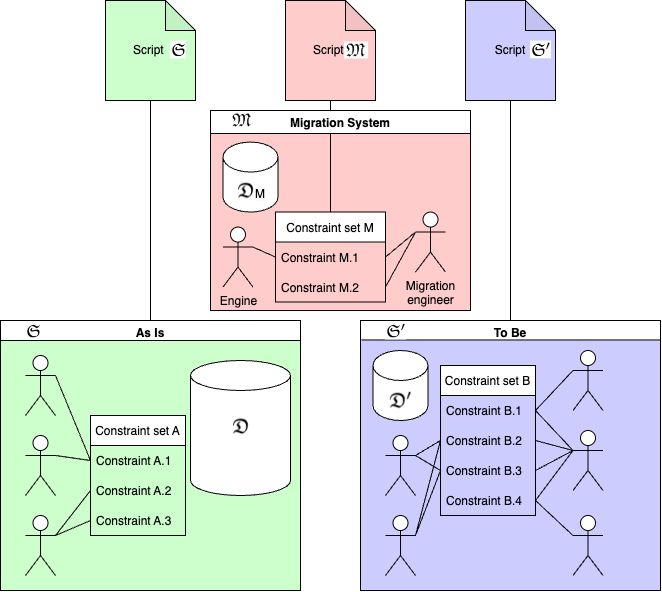
\includegraphics[scale=.45]{Migration.png}
   \end{center}
\caption{Data migration}
\label{fig:event flow}
\end{figure}
      
   We use two datasets: $\dataset$ and $\dataset'$.
   Before doing so, let us first define the disjoint union of two information systems.
\begin{definition}[disjoint union of datasets]
\begin{eqnarray}
   \omit\rlap{$\la\atoms,\concepts,\inst,\isa,\rels,\triples\ra\sqcup\la\atoms',\concepts',\inst',\isa',\rels',\triples'\ra$}\notag\\
   &=&\la\atoms\uplus\atoms',\ \concepts\uplus\concepts',\ \inst\uplus^2\inst',\ \isa\uplus^2\isa',\ \rels\uplus^3\rels',\ \triples\uplus^5\triples'\ra\notag\\
      X\uplus Y&=&\{(x,0)|\ x\in X\}\ \cup\ \{(y,1)|\ y\in Y\}\\
      X\uplus^2 Y&=&\begin{array}[t]{@{}l}\{((x_1,0),(x_2,0))|\ (x_1,x_2)\in X\}\ \cup\\ \{((y_1,1),(y_2,1))|\ (y_1,y_2)\in Y\}\end{array}\\
      X\uplus^3 Y&=&\begin{array}[t]{@{}l}\{\declare{(n,0)}{(A,0)}{(B,0)}\mid\ \declare{n}{A}{B}\in X\}\ \cup\\ \{\declare{(n,1)}{(A,1)}{(B,1)}\mid\ \declare{n}{A}{B}\in Y\}\end{array}\\
      X\uplus^5 Y&=&\begin{array}[t]{@{}l}\{\triple{(a,0)}{\declare{(n,0)}{(A,0)}{(B,0)}}{(b,0)}\mid\ \triple{a}{\declare{n}{A}{B}}{b}\in X\}\ \cup\\ \{\triple{(a,1)}{\declare{(n,1)}{(A,1)}{(B,1)}}{(b,1)}\mid\ \triple{a}{\declare{n}{A}{B}}{b}\in Y\}\end{array}
\end{eqnarray}
\end{definition}
Note that if $\dataset$ and $\dataset'$ are datasets, then so is $\dataset\sqcup\dataset'$.

\subsection{Example}
   Let us proceed to specify a to-be information system, $\infsys'$, to illustrate a (toy) migration.
   We will use the example in section~\ref{As-is IS} as the as-is information system
   and call that $\infsys$ in this section.
   Its population reflects the state of the information system just before the migration.

   Information system $\infsys'$, the to-be information system, is specified by:
\begin{verbatim}
   RELATION takes[Student*Course]
   RELATION isPartOf[Module*Course] [UNI]=
      [ ("IT-Governance", "Business IT") ]
   RELATION isEnrolledFor [Student*Module] =
      [ ("Susan", "Business Analytics")
      ; ("Susan", "IT-Governance")
      ; ("Susan", "Business Rules")
      ]
   RULE EnrollRule: isEnrolledFor |- takes;isPartOf~
   ROLE Administrator MAINTAINS EnrollRule
   
   RELATION course[ExamReg*Course] [UNI] =
      [ ("ER1", "Management")
      ; ("ER2", "Business IT")
      ; ("ER3", "Business IT")
      ]
   RELATION student[ExamReg*Student] [UNI] =
      [ ("ER1", "Peter")
      ; ("ER2", "Susan")
      ]
   RULE ExamRule1: student~;course |- takes
   RULE ExamRule2: student~;course;isPartOf~ |- isEnrolledFor
\end{verbatim}
   This specification shows that $\infsys'$ gets to keep all three relations and the rule from $\infsys$.
   Some new population, two new relations, and two new rules have been added to $\infsys'$.
   $\infsys'$ contains exam registrations (concept \verb-ExamReg-), which is new.
   In an exam registration, a student registers for the examination of a course.
   $\infsys'$ contains two extra rules: \verb-ExamRule1- and \verb-ExamRule2-.
   The first one says that an exam registration requires that a student actually takes the course.
   In logic, the constraint $p_{\tt ExamRule1}$ is written as:
\[\begin{array}{l}\forall s\in\text{\tt Student}, e\in\text{\tt ExamReg}, c\in\text{\tt Course}:\\
   e\ \text{\tt student}\ s\ \wedge\ \ e\ \text{\tt course}\ c\ \rightarrow\ s\ \text{\tt takes}\ c\\
\end{array}\]
   Another requirement, \verb-ExamRule2-, is that the student is enrolled for every module that is part of the course.
   Its constraint, $p_{\tt ExamRule2}$, is written in logic as:
\[\begin{array}{l}\forall s\in\text{\tt Student}, e\in\text{\tt ExamReg}, m\in\text{\tt Module}, c\in\text{\tt Course}:\\
   e\ \text{\tt student}\ s\ \wedge\ \ e\ \text{\tt course}\ c\ \wedge\ m\ \text{\tt isPartOf}\ c\ \rightarrow\ s\ \text{\tt isEnrolledFor}\ m
\end{array}\]
   Ampersand also derives the following violation sets:
\[\begin{array}{l}
   \viol{\text{\tt ExamRule1}}{\triples}\\
   \hspace{1cm}=\{\pair{s}{c}\mid\exists e:\ e\ \text{\tt student}\ s\ \wedge\ \ e\ \text{\tt course}\ c\ \wedge\neg(s\ \text{\tt takes}\ c)\}\\
   \viol{\text{\tt ExamRule2}}{\triples}\\
   \hspace{1cm}=\{\pair{s}{m}\mid\exists e,c:\ e\ \text{\tt student}\ s\ \wedge\ \ e\ \text{\tt course}\ c\ \wedge\ m\ \text{\tt isPartOf}\ c\ \wedge\neg(s\ \text{\tt isEnrolledFor}\ m)\}
\end{array}\]

   So let us now turn to the migration.
   The intention of any migration is to preserve as much of the data from $\infsys$ as possible into $\infsys'$,
   while adding the new triples to $\infsys'$.
   So the first thing to do is to take the disjoint union of both information systems.
   This yields:
\begin{verbatim}
   RELATION takes[Student*Course] =
      [ ("Peter", "Management")
      ; ("Susan", "Business IT")
      ; ("John", "Business IT")
      ]
   
   RELATION isPartOf[Module*Course] [UNI]=
      [ ("Finance", "Management")
      ; ("Business Rules", "Business IT")
      ; ("Business Analytics", "Business IT")
      ; ("IT-Governance", "Management")
      ; ("IT-Governance", "Business IT")
      ]
   
   RELATION isEnrolledFor [Student*Module] =
      [ ("Susan", "Business Analytics")
      ; ("Susan", "IT-Governance")
      ; ("Susan", "Business Rules")
      ]
   
   RULE EnrollRule: isEnrolledFor |- takes;isPartOf~
   ROLE Administrator MAINTAINS EnrollRule
   
   RELATION course[ExamReg*Course] [UNI] =
      [ ("ER1", "Management")
      ; ("ER2", "Business IT")
      ; ("ER3", "Business IT")
      ]
   RELATION student[ExamReg*Student] [UNI] =
      [ ("ER1", "Peter")
      ; ("ER2", "Susan")
      ]
   RULE ExamRule1: student~;course |- takes
   RULE ExamRule2: student~;course;isPartOf~ |- isEnrolledFor
\end{verbatim}
   If we check this for violations, we get the following results:
\begin{verbatim}
   There are 2 violations of RULE "ExamRule2":
      ("Peter", "IT-Governance")
      ("Peter", "Finance")
   ==============================
   There is one violation of RULE "UNI isPartOf[Module*Course]":
      ("IT-Governance", "IT-Governance")
\end{verbatim}
   Any data migration must anticipate any population in the as-is information system.
   The only thing we know for sure about the ``old'' population is that it satisfies the rules in $\infsys$.

\subsubsection{Strategies for dealing with violations}

The violations of ExamRule2 don't pose a problem: they have a role (administrator) assigned to them.
We allow these violations to occur in the transition to the new system, and expect people with the Administrator role to deal with them.

However, the violations that arise when taking the (non-disjoint) union of the two scripts include violations of rules that the information system should maintain.
This means that if we cannot generate software based on the disjoint union as it is.
To resolve this, the simplest solution is to change the roles assigned to the rules that are violated in the disjoint union:
\begin{verbatim}
   RELATION isPartOf[Module*Course]
   RULE isPartOfUNI: isPartOf;isPartOf~ |- I
   ROLE migrationHelper MAINTAINS isPartOfUNI
\end{verbatim}

Naturally, this solution requires effort from people with the role migrationHelper.
This in itself is not an issue: problems need to be solved one way or another.
However, a problem that may occur is that regular users of the system, who are used to the old system, might be adding data to the system that causes violations faster than they can be solved.
To mitigate this, we propose two solutions.

One solution is to state that the only violations that may occur in \verb=isPartOfUNI= are those that were present when the migration started:
\begin{verbatim}
   RELATION isPartOf[Module*Course]
   RULE isPartOfUNI: isPartOf;isPartOf~ |- I
   ROLE migrationHelper MAINTAINS isPartOfUNI
   
   RELATION isPartOfUNI_violations[Module*Module]
     = [("IT-Governance", "IT-Governance")]
   RULE isPartOfUNI_progress: -(isPartOf;isPartOf~) /\ I |- isPartOfUNI_violations
   SYSTEM MAINTAINS isPartOfUNI_progress
   
   ENFORCE isPartOfUNI_violations :< -(isPartOf;isPartOf~) /\ I  
\end{verbatim}

In this first solution, the first rule is the same as with the simple solution.
The second rule prevents any new violation from occurring.
Existing violations are recorded in the \verb=isPartOfUNI_violations= relation, and the rule \verb=isPartOfUNI_progress= prevents the set of violations to \verb=isPartOfUNI= from growing beyond this.
The \verb=ENFORCE= statement at the end of this code snippet states that the relation recording existing violations should be shrunk whenever violations are solved.
This way, we ensure that violations cannot re-occur.
As a whole, this means that \verb=migrationHelper= has a finite task.

As a second solution, we observe that the data in the designed system does not have any violations.
Consequentially, the cause of the violations comes from the triples in the old system.
Rather than taking the union of all triples, we can take the disjoint union instead;
\begin{verbatim}
   RELATION isPartOf_old[Module*Course] [UNI]=
      [ ("Finance", "Management")
      ; ("Business Rules", "Business IT")
      ; ("Business Analytics", "Business IT")
      ; ("IT-Governance", "Management")
      ]
   RELATION isPartOf[Module*Course] [UNI]=
      [ ("IT-Governance", "Business IT") ]
   RELATION isPartOf_ignored[Module*Course]
   
   RULE isPartOf_isUnion:  isPartOf_old :- isPartOf \/ isPartOf_ignored
   ROLE migrationHelper MAINTAINS isPartOf_isUnion
   
   ENFORCE isPartOf_ignored :> isPartOf
\end{verbatim}

\begin{verbatim}
   RELATION isPartOf_old[Module*Course] [UNI]=
      [ ("Finance", "Management")
      ; ("Business Rules", "Business IT")
      ; ("Business Analytics", "Business IT")
      ; ("IT-Governance", "Management")
      ]
   RELATION isPartOf[Module*Course] [UNI]=
      [ ("IT-Governance", "Business IT") ]
   RELATION isPartOf_ignored[Module*Course]

   ENFORCE isPartOf :> isPartOf_old - isPartOf_ignored
   ENFORCE isPartOf_ignored :> isPartOf
\end{verbatim}
In this second solution, we immediately move to a system in which the \verb=UNI= rule is maintained by the system.
The work for the \verb=migrationHelper= is again finite: the tuples in \verb=isPartOf_old= need to be copied over or explicitly ignored.
Once a tuple is in \verb=isPartOf=, the tuple is copied over to \verb=isPartOf_ignored= by the \verb=ENFORCE= statement, such that regular users can delete it without adding work to anyone with the \verb=migrationHelper= role.
Of course, since this solution starts with fewer pairs in the \verb=isPartOf= relation, other rules could be violated as a result of choosing this solution.
Indeed, ExamRule2 initially has more violations in this scenario.

\begin{definition}[migration dataset]
   \begin{eqnarray}
      &&\begin{array}[t]{@{}l}
         \{ {\tt ENFORCE\ }\declare{(nm',1)}{(A',1)}{(B',1)}\\\quad{\tt\ :=\ }\ident{(A',1)};\declare{(nm,0)}{(A,0)}{(B,0)};\ident{(B',1)}\\
            \mid\ \begin{array}[t]{@{}l}
               \declare{nm}{A}{B}\in\rels\wedge\declare{nm'}{A'}{B'}\in\rels'\wedge\id{nm}=\id{nm'}\ \wedge\\
               \{\pair{A}{A'},\pair{B}{B'}\}\subseteq\isa\cup\isa'\cup\flip{\isa}\cup\flip{\isa'}\}
               \end{array}
           \end{array}\\
           &\cup&\begin{array}[t]{@{}l}
            \{ {\tt CLASSIFY\ }(C',1){\tt\ IS\ }(C,0)|\ C\in\concepts,C'\in\concepts',C=C'\}\\
           \end{array}
   \end{eqnarray}
\end{definition}

The ${\tt CLASSIFY\ }(C',1){\tt\ IS\ }(C,0)$ statements add $((C',1),(C,0))$ and  $((C,0),(C',1))$ to the $\isa$ relation. Note that if $\dataset$ is a dataset, and $\dataset'$ is that dataset with pairs added\footnote{TODO: het woord `add' is informeel, dit kan beter} to the $\isa$ relation, then the result is again a dataset.
The ${\tt ENFORCE\ }r{\tt\ :=\ }e$ statements add triples $(x,r,y)$ for all $(x,y)\in e$.
The expressions $e$ in these statements are such that $x\ (\inst \compose \kleenestar{\flip{\isa}})\ (A',1)$ and $y \ (\inst \compose \kleenestar{\flip{\isa}})\ (B',1)$, thus preserving the property that the result is a dataset.

\begin{definition}[]
   \begin{eqnarray}
      \infsys\sqcup\infsys'&=&\la\roles',\rules',\maintain',\dataset\sqcup\dataset'\ra
   \end{eqnarray}
\end{definition}

\subsection{Changes}
% The purpose of this section is to explain why a dataset is structured the way it is.
   In the migration of a dataset we deal with changes to the elements that are not data:
   $\inst$, $\concepts$, and $\rels$.
   Such changes have further reaching consequences, however.
   Changes to $\inst$, $\concepts$, $\rels$ change the data structure in a dataset.
   We define a \define{migration of a dataset} $\la\atoms,\concepts,\inst,\rels,\triples\ra$ as a change in which one or more of $\inst$, $\concepts$, or $\rels$ change.
   To satisfy definition~\ref{def:dataset}, $\triples$ and $\atoms$ must change too,
   but the migration should try to preserve the maximal amount of data.

   This paper studies those changes and seeks to preserve the rules in definition~\ref{def:dataset}
   in such a way that large portions of migration can be automated.


\section{Bibliography}
\bibliographystyle{elsarticle-harv}
\bibliography{doc}


\end{document}
